\documentclass[thesis.tex]{subfiles}
\begin{document}

\chapter{Main}\label{chap:basics}

\section{Overview}
Our technique consists of three basic steps which are executed in every frame: Cache allocation, indirect lighting and cache interpolation.
The cache allocation pass assigns cells on a regular grid to cache memory.
Using a reflective shadow map, indirect lighting is then computed for all currently active cells.
Finally each pixel interpolates an indirect lighting value using all neighboring caches within the grid.

Each of the following major sections will explain one of these steps.
The last major section of this chapter will elaborate several implementation details, some of them crucial to the overall performance.\\
Many parts of our approach are based on several well-known techniques of which most have already been discussed in \autoref{chap:prevwork} and \autoref{chap:basics}.
Where necessary, details of the respective algorithms will be elaborated to address specifics implied by the overall technique.

\section{Cache Allocation}
Inspired by Lensing's LightSkin approach \cite{bib:LightskinPaper}, we wanted to compute indirect lighting only at specific locations instead at per-pixel frequency (as opposed to techniques like classic Reflective Shadow Maps or Voxel Cone Tracing).
\todo{detailed motivation to do that}
Since the goal of this work is a fully dynamic solution that works without any pre-computations, it is necessary to place such caches entirely at runtime.
\todo{definition of cache?}

\subsection{General Properties and Requirements of Dynamic Cache Placement}
There are several intrinsic advantages which can be expected of a dynamic light cache placement when compared to a precomputed placement.
Since we target for a single bounce of indirect light, caches are only used by currently visible locations (for multiple bounces it might be necessary to transfer lights between caches).
Also it should be possible to decrease the number of caches for distant objects, thus keeping the cache to screen-space density within a given bound.
Both properties result in a much lower memory footprint especially for large scenes when compared to precomputed solutions.

While it can be very beneficial to place caches dependent on the current few, this also may introduce several temporal artifacts, i.e. strong changes in indirect lighting from one frame to the next.
Additionally, target pixels need to have easy access to a certain number of caches to be able to interpolate them.
Note that such an apply pass can have temporal coherence problems on its own, as assignment of caches to surrounding world positions needs to be stable, no matter how densely they are sampled, i.e. by how many pixels an object covers.

So far, the data requirements of each cache were not defined.
Precomputed caches can naturally hold almost arbitrary data (within a given memory bound).
Dynamic caches on the other side need to refill theses data every frame, which is not only costly performance-wise but may also cancel out certain types of data as it may not be accessible. \todo{give an example? like lensing with area}
Naturally, such constraints also affect the following lighting and interpolation passes tremendously.

We evaluated several approaches before we came up with our final algorithm.
If you are interested you can read the summary of these attempts in \autoref{chap:abandoned}.

\subsection{Adaptive Cache Volume}
To cancel out temporal artifacts entirely, we decided to place caches only on the nodes of a regular grid in world space.
The main disadvantage of this method is, that cache are not placed on surfaces and thus have no concrete orientation.
This means that all information must be function on or completely independent of the surface normals.

During the cache allocation pass, each pixel activates its eight nearest caches.
This can be easily done by a fullscreen pass, using the depth buffer from the previously rendered scene.
\todo{write: allows for optimizations since neighboring pixels activate the same cache - see blabla}

The grid moves with the view frustum to cover it entirely.
Movements need to be performed in discrete steps, equaling the distance between two caches, since smooth movements would lead again to temporal incoherences.

Even so, usually only a very small fraction of all grid cells contains an activated cache.
To save memory, we use a \emph{address volume} that contains only an integer per cell which serves as a pointer to the actual cache data which lies in a separate buffer.
Since the position of a cache can no longer be deduced by its memory position, the position needs to be saved within each cache.
Using an address volume not only reduces memory computation drastically, it makes it also much easier to perform the lighting for each active cache which do now lie consecutive in memory instead of scattered within a volume.


\section{Indirect Lighting}
The indirect lighting of the caches relies on reflective shadow maps (see \todo{citation needed}).
In principle each cache iterates on the entire RSM to retrieve the encoded indirect lighting informations.
The following chapters explain how this information is processed and how the results are saved for later interpolation.

\subsection{Diffuse Lighting}
Diffuse lighting is handles straight forward.
Each RSM pixel is interpreted as a disc-shaped light as described by Lensing (see \todo{either explain here or earlier}).
The total irradiance per normal is summed up into a low-order spherical harmonics representation.

Using zonal harmonics, the irradiance contribution of a single light to the spherical harmonics coefficients can be computed analytically.
Assume that the direction to the light would be $(0,0,1)$, then the irradiance 
\begin{equation}

\end{equation}


\subsection{Specular Lighting}


\subsection{Indirect Shadows}

\subsubsection{Scene Voxelization}

\subsubsection{Cone Casts on Filtered Reflective Shadow Maps}


\section{Cache Interpolation}



\section{Implementation}

\emph{As many as possible details should be delayed into this chapter. If it gets large or starts to mirror the main part, make it a chapter!}

This is the right place for describing how to use Compute, OpenGL etc. for achieving the rather abstract formulated goals of the sections before.

Deferred Renderer, 32bits per Layer RGB(A) srgb - Diffuse, RG 16snorm - Normals with angles, extra infos todo, R32F Depth Buffer (swapped near/far)\\
(This detail belongs more or less to Eva...)

\subsection{Pipeline Overview}

\begin{figure}[h]
	\centering
	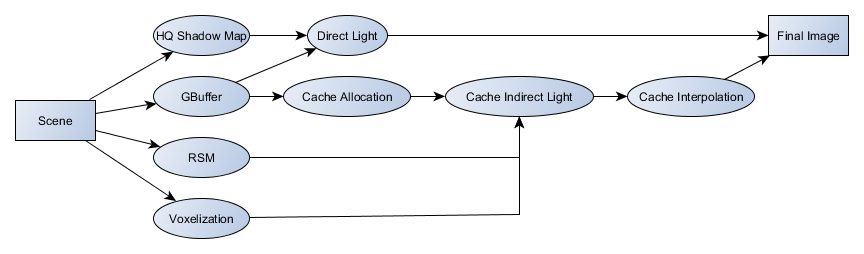
\includegraphics[width=\textwidth]{renderingpipeline_draft}
\end{figure}

\todo{same with image}

\todo{explanation}

\subsection{Cache Allocation}
cacheList via shared memory etc.
"Adress Coord Cache"

\subfilebib % Makes bibliography available when compiling as subfile
\end{document}